\chapter{User interface}

A \emph{user interface} (UI) is the front-facing part of Pepr3D that the users are going to interact with.
It is responsible for managing windows, showing buttons, texts, rendering the 3D model, handling mouse clicks, and much more.
In case of Pepr3D, it needs to be a cross-platform, easy-to-use, intuitive, and fast abstraction of the complex 3D geometric algorithms at the backend, see Figure~\ref{fig:architecture_ui}.

\begin{figure}[h]
	\centering
	\centerline{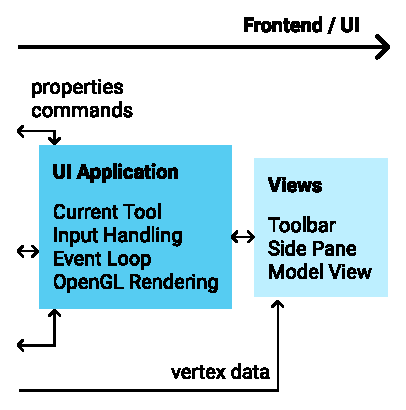
\includegraphics[scale=0.9]{images/architecture_ui.eps}}
	\caption{An overview of the Pepr3D UI architecture, based on Figure~\ref{fig:architecture}.}
	\label{fig:architecture_ui}
\end{figure}
\vspace{-1.5em}
\section{Introduction}

We did not want to reinvent the wheel, so we investigated how other developers recommend to implement user interfaces.
In our case, we have \emph{3D rendering}, i.e., displaying the 3D model, and \emph{UI widgets}, i.e., the windows, buttons, check boxes, text labels, etc.
Here we describe what we found important to understand.

\subsection{Existing patterns}

Let us have a look at existing generic UI architectural patterns.
A detailed overview of them was written for example by Derek Greer\footnote{https://lostechies.com/derekgreer/2007/08/25/interactive-application-architecture/}.
The most common pattern is called Model-View-Controller (MVC), where \emph{model} is a state, \emph{views} visualize the state, and \emph{controllers} react to user input to manipulate the model.
The MVC pattern got so famous that there are a lot of alternatives nowadays based on the similar principles, like Model-View-Viewmodel (MVVM), Model-View-Presenter (MVP), or Presentation-Abstraction-Control (PAC).

But we can go even further: Johannes Norneby mentions\footnote{http://www.johno.se/book/immvc.html} a common paradigm of UI, which he objects is \emph{not valid}: \emph{``The user interface and / or visualization of any program is inherently stateful.''}
He objects that this is a broken paradigm and devotes his book into explaining the so called \emph{immediate user interface}, which instead provides a \emph{stateless} alternative to rendering UI.
% Nowadays, there exist various libraries and frameworks based on this idea, the most well known probably being ImGUI\footnote{https://github.com/ocornut/imgui} supported by large companies such as Blizzard Entertainment.

The main difference between \emph{immediate} and \emph{retained} modes is that in the latter, the visualization library \emph{retains} internally a complete model (state) of objects to be rendered, while the former is procedural and redrawn every frame.\footnote{http://msdn.microsoft.com/en-us/library/windows/desktop/ff684178(v=vs.85).aspx}
The major benefit of a stateless immediate UI is the ability to maintain and reuse it much easier.
Norneby suggests that every \emph{view} should be as \emph{pure} as possible, meaning that in languages like C++, all views should in fact be \emph{free functions}.

\subsection{Immediate vs. retained}

Even when one sticks to MVC principles, there does not seem to be a consensus for which applications one should prefer the \emph{retained} mode over \emph{immediate} and vice versa.
At its core, MVC principles can be used in both of them.
Norneby goes as far as saying that MVC \emph{and} immediate UI are two implicitly connected concepts.
Arguments were made\footnote{https://gamedev.stackexchange.com/questions/24103/immediate-gui-yae-or-nay} for both approaches without a clear winner.

The main downside of retained UI is the necessity to maintain a UI state.
This often leads to complex libraries that are difficult to learn to work with and introduces out-of-sync bugs that are hard to fix.
This is why video game and interactive applications developers (including Blizzard Entertainment) support immediate UI, because it \emph{interlocks} the application data and the current state of the UI, meaning the state and UI never get ouf of sync.
The libraries are also usually very simple to use.

The main downside of immediate UI is a poor separation of logic and presentation and the necessity to rerender the UI more often.
What developers at uiink\footnote{https://uiink.com/articles/data-driven-immediate-mode-ui/} suggest is to just use the best of the both worlds.
And it is not different from what Norneby actually proposed in his never-finished book.
We should only use immediate UI in the actual \emph{views}, which are just free functions procedurally explaining how the UI should be rendered each frame.
The rest of the application should know nothing about immediate UI.
In theory, we should be able to swap immediate UI and retained UI, or use both of them together without the need to touch the rest of the application.

\subsection{Real-time rendering}

In Pepr3D, a regular user interface with a few buttons and texts is not enough.
We primarily need real-time 3D rendering and manipulation of the 3D model that the user is editing.
Hence the whole user interface needs to take this into account and should be primarily based on real-time rendering.

As already mentioned, real-time applications such as video games favor immediate UI.
They need to rerender the whole screen all the time anyway.
For Pepr3D, it is perfectly possible to make immediate UI a part of the renderer.

\subsection{Presentation separated from logic}

Nowadays, a lot of UI is being developed for web applications.
We can investigate the most used frameworks and libraries for single-page applications\footnote{React: https://reactjs.org/, Angular: https://angular.io/, Vue.js: https://vuejs.org/}: React by Facebook, Angular by Google, or Vue.js.

We observed that these tend to follow the principle that a \emph{view should be just a thin front-facing layer only responsible for displaying data}.
Calculations and data manipulation should be done in other parts of the application.

It is not a surprise that even Qt\footnote{https://www.qt.io/}, a widely used C++ UI framework, encourages people to eliminate data consistency problems by using separate \emph{views}.\footnote{http://doc.qt.io/qt-5/modelview.html}
Even though there are so many different UI libraries and frameworks, they all seem to share the same common principles about the separation of presentation.

\subsection{Internationalization and accessibility}

There are many other observations one can make when studying existing applications that heavily rely on user interface.
A lot of energy has been invested into creating standards and guidelines for them.
It is not in the scope of this work to list all details about building good user interfaces, but we should still mention at least two more concepts: internationalization and accessibility.

Typically, when applications are used by users from different countries, the UI needs to support \emph{internationalization} (abbreviated as \emph{i18n})\footnote{https://blog.mozilla.org/l10n/2011/12/14/i18n-vs-l10n-whats-the-diff/}, i.e., different languages, number formats, time formats, etc.

Applications should also be \emph{accessible} (accessibility, abbr. \emph{a11y}), meaning they should support keyboard navigation for people who cannot use mouse, screen readers for people who are blind, high contrast themes for people with worse eyesight or color blind users, etc.
Especially in the ``web world'', there exist important accessibility guidelines called WCAG.\footnote{https://www.w3.org/WAI/standards-guidelines/wcag/}

\section{Our requirements}\label{sec:uireqs}

Based on the observations made in the previous section, on the expected usage of our application, and on general advice gathered from Vojtěch Bubník from Prusa Research s.r.o., we decided on the following set of requirements for the user interface of Pepr3D.

The user interface of Pepr3D and the library we are going to use for it should:
%
\begin{enumerate}
\setlength\itemsep{0em}
\item separate presentation from application logic, i.e., in theory, we should be able to easily replace the UI with another one, should it be necessary,
\item support real-time 3D rendering of the 3D model, provide an easy-to-use abstraction, e.g., for rendering 3D primitives, using custom shaders with uniforms, uploading textures to the GPU, keeping constant framerate, etc.,
\item look visually good and allow us to unify the design of the 3D rendering part and the rest (toolbar, controls, etc.), e.g., by supporting custom themes,
\item be cross-platform at least on desktop (Windows, Mac, Linux), ideally on tablets as well (Android, iOS), i.e., the ``cross-platformity'' of Pepr3D should not be limited by the UI library,
\item support keyboard navigation, e.g., tabbing to buttons and input elements, using keyboard to enter values,
\item support high DPI, e.g., Apple Retina displays, Microsoft Windows scaling,
\item support asynchronous events, e.g., long calculations on background should not affect the UI thread,
\item support internationalization including plurals, time formats, UTF-8, and
\item the license of such library should be as least restrictive as possible, e.g., allowing commercial usage and redistribution, should the development of Pepr3D continue after this initial school project is finished.
\end{enumerate}

\section{Choosing a 3D rendering library}

There are many cross-platform C++ libraries for 3D rendering and for creating user interfaces.
Picking the right ones for Pepr3D is not an easy task.
Fortunately, as we built a list of requirements in the previous section, we can easily disregard the libraries that do not conform to our requirements.
Let us now describe how we chose a library for the 3D rendering part of Pepr3D.

\medskip

In order to support multiple platforms and even older computers, we decided to use OpenGL rendering API instead of Microsoft DirectX or alternatives like Vulkan.
We cannot use OpenGL on its own as we need a library to handle cross-platform windows, contexts, keyboard and mouse inputs, etc., so it is necessary to find a library that can help us with that.

There are many libraries like SDL, GLFW, Cinder, Ogre3D, or bgfx,\footnote{https://www.libsdl.org/, https://www.glfw.org/, https://libcinder.org/, https://www.ogre3d.org/, https://github.com/bkaradzic/bgfx} and some UI libraries like Qt can also help with that.
Some of these libraries depend on others from the list, for example bgfx uses SDL for windows and input handling, and Cinder uses native code for Windows and OS X but GLFW on Linux.

We had previous knowledge of Cinder and bgfx.
The other libraries we examined did not seem to provide any advantages over these two, either because they were already included in the two, or because they were too heavy.

We found that Cinder conforms to our requirements better than bgfx:
Cinder has built-in high DPI support, font rendering, event loop for asynchronous events, a big set of tutorials and examples, and much more.
We have decided to choose \textbf{Cinder} as the library for real-time 3D rendering.

\section{Choosing a UI widgets library}

Now that we know what library to use for 3D rendering, we need to choose a way to display \emph{widgets} such as toolbars, buttons, check boxes, or text labels.
Again, there are famous cross-platform libraries that already exist for these purposes, so it would not make much sense to make our custom solution.

\subsection{Why not wxWidgets nor GTK$+$}

We should definitely mention retained UI libraries wxWidgets and GTK+.\footnote{https://www.wxwidgets.org/, https://www.gtk.org/}
They are both cross-platform and used by famous software like GIMP or Audacity.
Unfortunately, we found major flaws with both of them.

Regarding wxWidgets, we did not really like its default appearance.
It uses native controls where possible making theming very limited and also undocumented.
Hence, we would not be able to easily unify the design of the 3D view and the rest of the application.
Also, only desktop is supported.

Regarding GTK+, they do support theming up to some degree, they also added OpenGL rendering widgets a few years ago.
Making Cinder and GTK+ work together would probably cost us some effort as we did not find any already working solution.
The problem with GTK+ is that a lot of developers who actually use it are not satisfied and warn others about using it.\footnote{https://davmac.wordpress.com/2016/07/05/why-do-we-keep-building-rotten-foundations/}$^{,}$\footnote{https://fosspost.org/opinions/are-gtk-developers-destroying-linux-desktop-with-their-plans}$^{,}$\footnote{https://www.reddit.com/r/linuxmasterrace/comments/7xkcwo/}

They say that GTK+ documentation is very bad and that different versions of GTK+ break existing applications, extensions, and themes, because the API and ABI is changing rapidly providing no guarantees.
It did not seem that using GTK+ for Pepr3D would be a good long-term idea should anyone continue with its development in the future.

\subsection{Qt}

We have already mentioned Qt on previous pages of this specification.
It is a rather large actively-developed library providing a lot of features including their own internationalization solutions and so on.
Qt conforms to all our requirements stated in the previous section.
There are two major drawbacks with Qt: its controversial licenses\footnote{https://www1.qt.io/licensing-comparison/} and its huge size.

The licensing is controversial because either one can pay for the commercial license, or one can use the LGPLV3 one, but it requires dynamic linking, providing users the ability to relink the application, and also the necessity to deliver complete Qt source codes to users including all changes made if any.
The huge size is also an issue, because using only the basics of Qt (widgets, GUI, and core) is already around 17 megabytes in libraries, which together with Cinder would lead to a very large size of the final Pepr3D application.
It is also uncertain whether it would be a good idea to use Cinder together with Qt, so we would possibly need to rely on a different library.

\subsection{UI libraries for OpenGL}

There are also libraries that do not use native controls at all, but rather generate draw instructions and lists that can be used by renderers like OpenGL directly.
The libraries itself do not handle window creation, native calls to operating systems, etc.
Users of such a library need to bind the input handling and draw commands of these libraries to their own OpenGL/DirectX/other renderer.
In our case, we would need to connect the library to Cinder, which handles windows, inputs, and rendering itself.

There are many such libraries, e.g., Dear ImGui, Nuklear, NanoGUI, and FlatUI.\footnote{https://github.com/ocornut/imgui, https://github.com/vurtun/nuklear, https://github.com/wjakob/nanogui, https://github.com/google/flatui}
While some of them like NanoGUI and FlatUI seem to be rather small, without that many users, and not under active development, Nuklear and Dear ImGui are still under active development and maintenance.

Nuklear is an ANSI C header-only library with a C API and C naming conventions.
We did not manage to find existing Cinder--Nuklear bindings that we would be able to use, so we would need to develop them ourselves.
For this reason, we did not continue investigating Nuklear, because we found an alternative.

Dear ImGui (or just ImGui) is a modern bloat-free C++11 library that we already mentioned in the previous sections.
It is backed by large companies like Blizzard Entertainment or NADEO.
Its community is very active providing different bindings for different renderers and libraries including Cinder.
It is easily themable and we have created a prototype with completely custom controls.

\subsection{Final decisions}

For our final decisions, we have selected two libraries: \textbf{Qt} and \textbf{ImGui}.
When looking at our requirements from Section~\ref{sec:uireqs} (numbering refers to Section~\ref{sec:uireqs}):
%
\begin{enumerate}
\setlength\itemsep{0em}
\item separation can easily be achieved in both using Views and Models,
\item OpenGL rendering is implicit in ImGui, there is a widget in Qt,
\item theming in Qt: QSS stylesheets, in ImGui: styles and custom drawing,
\item both are cross-platform even on mobile devices,
\item both support keyboard navigation, ImGui since version 1.60,
\item high DPI possible in Qt, for ImGui we can use Cinder high DPI support,
\item Qt has its own thread pool, signals, and promises, for ImGui we can use C++11 and Cinder/ASIO event loop using dispatchAsync,
\item Qt has its own i18n support, for ImGui we can use PO files and gettext\footnote{Free i18n system commonly used on Linux, see https://www.gnu.org/software/gettext/} together with a translation editor, e.g., open-source PoEdit\footnote{https://poedit.net/},
\item Qt is unfortunately commercial or LGPLV3 (see above), ImGui has much less restrictive MIT License.
\end{enumerate}

As we can see, there is no clear winner: both libraries have positive and negative attributes.
In fact, Qt and ImGui are very different.
Qt is a large retained UI library and ImGui is a small bloat-free immediate UI library.

Using Qt together with Cinder is rather questionable as they both overlap in certain areas like window management and event handling.
Whereas ImGui needs a renderer and a window handler anyway, so using it with Cinder seems to be a good idea.
ImGui is much closer related to the actual OpenGL rendering and offers us quite a bit more flexibility.
It also has a very simple source code that one can read in an evening, meaning we can actually learn a lot about how such a library is made.

We think that Qt would probably be an unecessary huge piece of middleware that we would have to learn just for the sake of this project.
We have decided to use \textbf{ImGui} for the Pepr3D user interface.

\section{Final proposal}

In Section~\ref{sec:wireframe} and in Figure~\ref{fig:wireframe}, we have already proposed a wireframe of Pepr3D and explained why we find it reasonable and easy to use.
In this chapter, we explained our requirements and investigated existing patterns for actually implementing the UI.
Let us now propose how we can use these together.

\subsection{Overview}

We propose to divide the Pepr3D UI into the following main parts that correspond to the wireframe in Figure~\ref{fig:wireframe} and to Figure~\ref{fig:uioverview}:
%
\begin{itemize}
\setlength\itemsep{0em}
\item a \textbf{toolbar} with toggleable buttons representing tools, undo/redo, etc., implemented as an ImGui widget rendered with Cinder,
\item a \textbf{side pane} with buttons, checkboxes, sliders, etc., representing configuration of the currently selected tool, also implemented as an ImGui widget rendered with Cinder,
\item and a \textbf{model view} with the 3D model which the user can rotate, zoom, paint on it, etc., implemented in OpenGL using Cinder.
\end{itemize}

Even though the toolbar and side pane are to be implemented in ImGui, they will in fact be rendered using Cinder and OpenGL as well.
The whole window is managed by Cinder and has a single large OpenGL drawing context.

\begin{figure}[h]
	\centering
	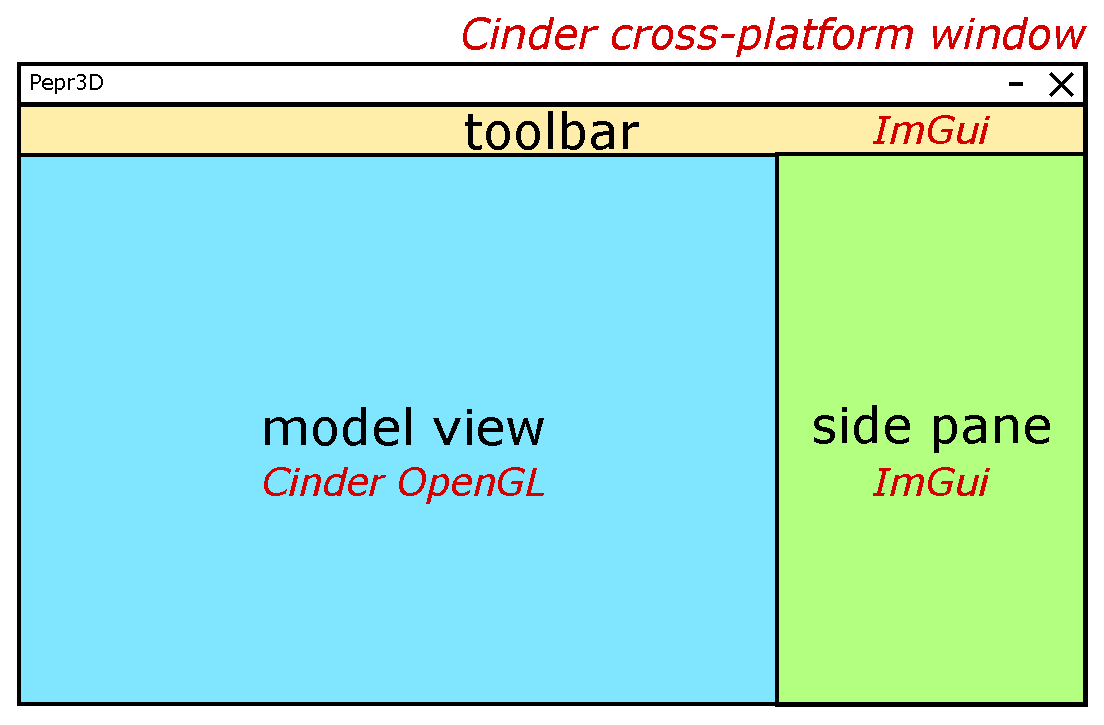
\includegraphics[scale=0.65]{images/uioverview.eps}
	\caption{An overview of the Pepr3D UI.}
	\label{fig:uioverview}
\end{figure}

\vspace{-1em}
\subsection{Stateless views / widgets}

Inspired by the immediate UI advice, we propose to use \emph{stateless views} that will be responsible for drawing the UI.
We can implement these views as C++ free functions without encapsulating them in any classes.
This is a common pattern in C++, e.g., in the standard library, because unlike in languages like Java and C\#, functions in C++ do not need to be enclosed in classes.

Having stateless views means that we do not have to program any explicit synchronization between the UI and the backend.
Whenever we rerender the UI, it will be rendered with the newest data.
We should try to avoid retained state in the UI as much as possible, but it might be necessary in specific situations, e.g., for scrollbar positions or complex calculations that we do not want to do each frame.
The ImGui library provides ways for retaining states.
Where necessary, we can also use regular C++ classes and their instances.

There is also a huge ImGui community at GitHub, where we can find both simple and complex widgets available from other users of the library.
We should aim at making our UI composed of reusable ImGui widgets.

\subsection{Internationalization and accessibility}

It should be possible to change a language of the application.
For this purpose, we propose to use PO files that are used by a lot of Linux distributions and applications including PHP.
Loading the PO files can be handled by lightweight libraries that already exist and are suitable for our project, at a first glance sporit-po\footnote{https://github.com/cbeck88/spirit-po} looks perfect for our purposes.
The files themselves can be generated from source codes and translated using for example the already mentioned PoEdit.

The UI should provide basic keyboard navigation including hotkeys (shortcuts).
It is especially important that the currently selected tool can be changed by pressing a single key on a keyboard.
We also considered adding a radial menu to a specific mouse button (e.g., middle button click), but it is not a top priority.
The default theme of Pepr3D should provide sufficient contrast and it should be easy to see which tool is selected and what options are enabled.
